%%%%%%%%%%%%%%%%%%%%%%%%%%%%%%%%%%%%%%%%%%%%%%%%%%%%%%%%%%%%%%%%%%%%%%%%%
%
% File: Model.tex
%
% Purpose: Top level document for Model.  Should not need to be edited.
%
%%%%%%%%%%%%%%%%%%%%%%%%%%%%%%%%%%%%%%%%%%%%%%%%%%%%%%%%%%%%%%%%%%%%%%%%%

\documentclass[twoside,11pt,titlepage]{report}

%
% Bring in the common page setup
%
\usepackage{dynenv}

%
% Bring in the model-specific commands
%
\usepackage{PLANETFIX}

%
% Bring in the graphics environment
%
\usepackage{graphicx}
\usepackage{appendix}
%
% Bring in the hyper ref environment
%
\usepackage[colorlinks,plainpages=false]{hyperref}
%  keywords for pdfkeywords are separated by commas
\hypersetup{
   pdftitle={\PLANETFIXDesc},
   pdfauthor={\ModelAuthor},
   pdfkeywords={\ModelKeywords},
   pdfsubject={\PLANETFIXDesc}}

% for document revisions only:
\newcommand\documentHistory{
{\bf Author} & {\bf Date} & {\bf Description} \\ \hline \hline
A. A. Jackson and J. Morris & October 2009 &  Initial Version \\ \hline
A. A. Jackson and J. Morris & December 2009 & Revision \\ \hline
R. O. Shelton & January 2011 & Revision \\ \hline
}


\begin{document}

%%%%%%%%%%%%%%%%%%%%%%%%%%%%%%%%%%%
% Front matter
%%%%%%%%%%%%%%%%%%%%%%%%%%%%%%%%%%%
\pagenumbering{roman}

\docid{models/utils/planet\_fixed}
\docrev{1.0}
\date{\RELEASEMONTH\ \RELEASEYEAR}
\modelname{\PLANETFIXDesc}
\doctype{}
\author{\ModelAuthor}
\managers{
  Robert O. Shelton \\ Project Manager \\
  Michael T. Red \\ Simulation and Graphics Branch Chief \\
  R. Matt Ondler \\ Software, Robotics, and Simulation Division Chief}
\pdfbookmark{Title Page}{titlepage}
\makeDynenvTitlepage

\pdfbookmark{Abstract}{abstract}
%%%%%%%%%%%%%%%%%%%%%%%%%%%%%%%%%%%%%%%%%%%%%%%%%%%%%%%%%%%%%%%%%%%%%%%%
%Planet Fixed Utility
% Purpose:
%
% 
%
%
%%%%%%%%%%%%%%%%%%%%%%%%%%%%%%%%%%%%%%%%%%%%%%%%%%%%%%%%%%%%%%%%%%%%%%%%%

\begin{abstract}
This model utility provides two coordinate transformations:
\begin{itemize}
\item A module for transformation from planet centered planet fixed Cartesian coordinates to
      planetospherical or planetoellipsoidal coordinates (a longitude, latitude, altitude set)
      and vice versa.(Note: in the model the word ellipse occurs in place of ellipsoidal coordinates.
      The reader should note that ellipsoidal is the standard usage for a given planetary body.
       See the Explanatory Supplement to the Astronomical Almanac \cite{Seidelmann}.
\item A module for transformation from planet centered planet fixed to a tangent plane system.
      This is a horizon system and here is chosen to be the North East Down specification with
      coordinates of altitude , latitude (or elliptical latitude) and longitude chosen as the non
      cartestian coordinates.(This is the reversed version of Local North East Up coordinates, where height
      (or altitude), right ascension and declination are chosen.)
\end{itemize}
The term planet\_fix refers to the two utility modules planet\_fixed\_posn and north\_east\_down.\\
These coordinates and coordinate transformation apply to any body in the solar system. The reader however
will find difference nomenclature in the literature for these as noted above.
\end{abstract}

\setcounter{chapter}{0}
\pdfbookmark{Contents}{contents}
\tableofcontents
\vfill
%----------------------------------
\chapter{Introduction}\hyperdef{part}{intro}{}\label{ch:intro}
%----------------------------------
\pagenumbering{arabic}

\section{Model Description}
This model is a utility with JEOD to provide transformations between Cartesian , Spherical , Spheroidal and
Tangent Plane coordinates. It is made up of two modules Planet Fixed and North East Down (a tangent plane system).

\section{Document History}
%%% Status of this and only this document.  Any date should be relevant to when
%%% this document was last updated and mention the reason (release, bug fix, etc.)
%%% Mention previous history aka JEOD 1.4-5 heritage in this section.
%%% Mention that JEOD.pdf is the parent document.

\begin{tabular}{||l|l|l|} \hline
\documentHistory
\end{tabular}



This document is formatted in accordance with the
NASA Software Engineering Requirements Standard~\cite{NASA:SWE}
and is organized into the following chapters:


\section{Document Organization}
This document is formatted in accordance with the
NASA Software Engineering Requirements Standard~\cite{NASA:SWE}
and is organized into the following chapters:

\begin{description}

\item[Chapter 1: Introduction] -
JEOD has the capability to take a position
vector in one coordinate system, and convert it to
another coordinate system. JEOD has several coordinates systems,
in the following focus is on two modules under the utility planet\_fixed.
There are four coordinate systems to consider, planet centered planet fixed Cartesian,
planet fixed spherical, planet fixed elliptical and a tangent plane coordinate system.
In  this document for all planet fixed coordinates, no epoch has been specified, the fiducial
reference is the prime meridian and the mean rotational axis of a planet. This module is
meant to be generic and a reference body planet, satellite or other solar system body must
be specified.

\item[Chapter 2: Product Requirements] -
Describes requirements for the \PLANETFIXDesc.

\item[Chapter 3: Product Specification] -
Describes the underlying theory, architecture, and design of the \PLANETFIXDesc\ in detail.  It is organized in
three sections: Conceptual Design, Mathematical Formulations, and Detailed Design.

\item[Chapter 4: User Guide] -
Describes how to use the \PLANETFIXDesc\ in a Trick simulation.  It is broken into three sections to represent the JEOD
defined user types: Analysts or users of simulations (Analysis), Integrators or developers of simulations (Integration),
and Model Extenders (Extension).

\item[Chapter 5: Verification and Validation] -
Contains \PLANETFIXDesc\ verification and validation procedures and results.

\end{description}

%----------------------------------
\chapter{Product Requirements}\hyperdef{part}{reqt}{}\label{ch:reqt}
%----------------------------------
\requirement{Implement a set of planet fixed coordinates in \JEODid}
\label{reqt:pfix}
The requirement for the various planet fixed coordinate systems is to define the following coordinate systems and
implement the ability to transform to and from each. Note: 'Fixed' is the astrodynamic specification for a coordinate
system rotating with associated celestial body.
The coordinate systems are:
\subrequirement{Planet fixed Cartesian}\label{reqt:pfixcart}\ \newline
\begin{itemize}
\item Planet fixed Cartesian:
\begin{enumerate}
\item X-axis: The intersection of the prime meridian and the rotation equator of the named solar system object (planet, satellite, asteroid)
\item Y-axis: Completes a standard, right-handed coordinate frame named solar system object (planet, satellite, asteroid)
\item Z-axis: The mean rotation pole of the named solar system object (planet, satellite, asteroid)
\end{enumerate}

\subrequirement{Planet fixed spherical}\label{reqt:sphere}\ \newline
\item Planet fixed spherical
\begin{enumerate}
\item Altitude ~h - The height above a given equatorial radius of the named solar system object (planet, satellite, asteroid)
\item Longitude {$\lambda$}  - Is angle measured along the mean equator positive east from the prime meridian of the named solar system object (planet, satellite, asteroid)
\item Spherical Latitude {$\theta$}  -  Is the angle measured from the mean equator positive north of the named solar system object (planet, satellite, asteroid)
\end{enumerate}
\begin{figure}[htp]
\centering
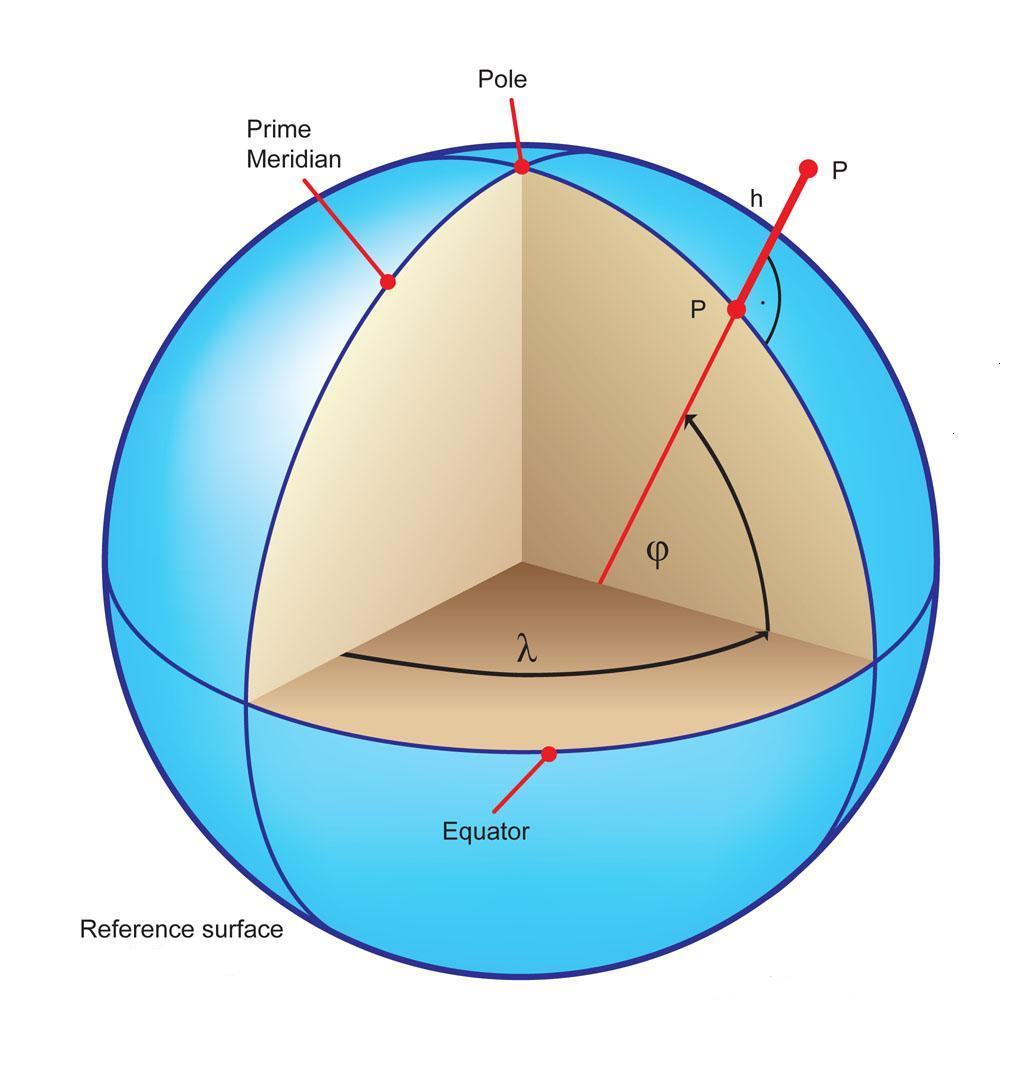
\includegraphics [width=7in]{figs/lonlat.jpg}
\caption{Prime meridian planet fixed}
\label{fig:1}
\end{figure}


\subrequirement{Planet fixed Elliptical}\label{reqt:pfixellip}\ \newline
\item Planet fixed elliptical
\begin{enumerate}
\item Height {h} - At a point is the distance from the reference ellipsoid*\ref{elip}, see figure \ref{fig:2} to the point in a direction normal of the reference ellipsoid of the named solar system object (planet, satellite, and asteroid)
\item Latitude elliptical {$\theta$} - Is the angle between the equatorial plane and a line that is normal to the reference ellipsoid of the named solar system object (planet, satellite, and asteroid)
\item Longitude {$\lambda$} - Is angle measured along the mean equator positive east from the prime meridian of the named solar system object (planet, satellite, asteroid)
*\label{elip} A reference ellipsoid is defined by semi-major (equatorial radius) and flattening (the relationship between equatorial and polar radii of the named solar system object (planet, satellite, and asteroid).
\end{enumerate}

\begin{figure}[htp]
\centering
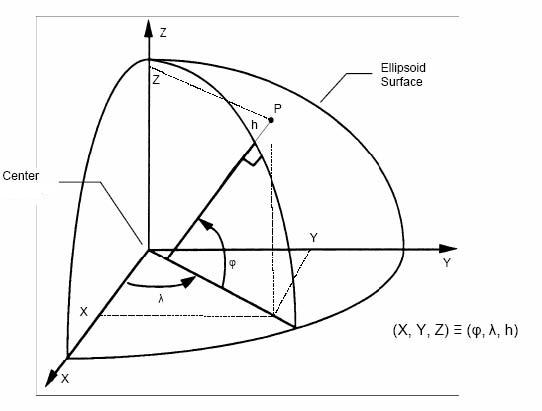
\includegraphics [width=5in]{figs/ellipse.jpg}
\caption{Planet fixed ellipsoid system}
\label{fig:2}
\end{figure}

\newpage

\subrequirement{Planet fixed tangent plane}\label{reqt:pfixtan}\ \newline
\item Local Planet fixed tangent plane can be associated with either a spherical or an elliptical coordinate system.
A tangent plane is attached to a fixed point on an elliptical (or spherical) surface a named solar system object (planet, satellite, and asteroid)see figure \ref{fig:3}.
\begin{enumerate}
\item x component of the coordinate (NORTH)
\item y component of the coordinate (EAST)
\item z component of the coordinate (UP)
\end{enumerate}
\end{itemize}

\begin{figure}[htb]
\centering
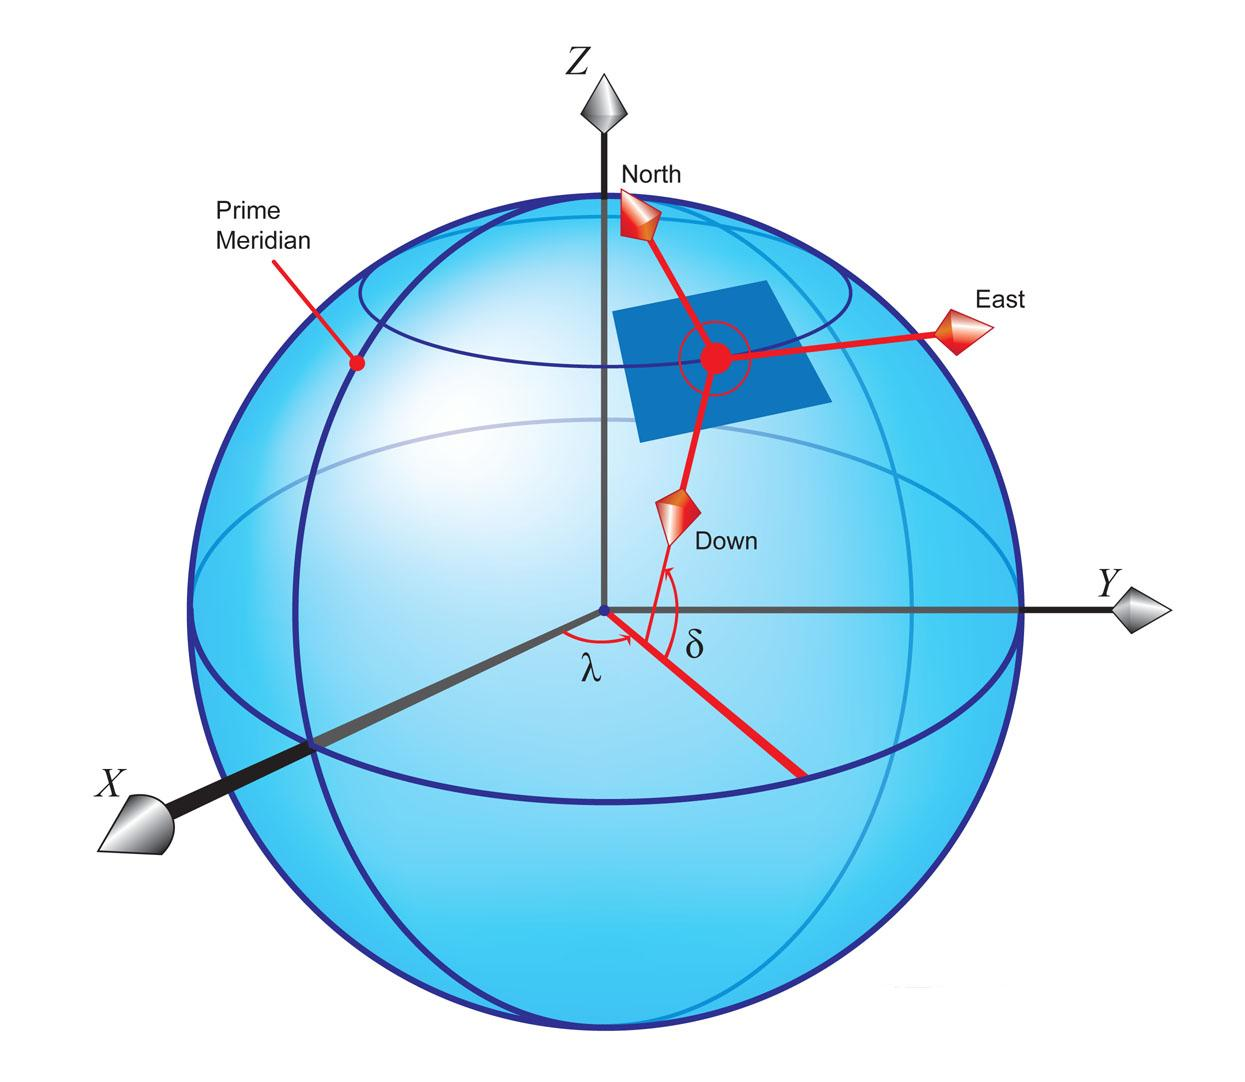
\includegraphics [width=4in]{figs/tan.jpg}
\caption{Local planet fixed tangent plane}
\label{fig:3}
\end{figure}

%----------------------------------
\chapter{Product Specification}\hyperdef{part}{spec}{}\label{ch:spec}
%----------------------------------

\section{Conceptual Design}
JEOD coordinate systems are generic in that any given solar system body (or bodies) one or several can be specified.
For the Planet Fixed modules a set of four coordinate systems are specified.
For solar system bodies the IAU differentiates between Planet Centered and planetographic body-fixed coordinates : Planet Centered latitude refers to the equatorial plane and the polar axis, planetographic latitude is defined as the angle between equatorial plane and a vector through the point of interest that is normal to the biaxial ellipsoid reference surface of the body. Both latitudes are identical for a spherical body. Planet Centered longitude is measured eastwards (i.e. positive in the sense of rotation) from the prime meridian. Planetographic longitude of the sub-observation point increases with time, i.e. to the west for prograde rotators and to the east for retrograde rotators.

Note in the following the terms spherical will be used for Planet Centered and elliptical for planetographic. The planet
fixed tangent plane is the nominal 'local horizon's system defined here in 'aeronautic' terms of north east and down.

\section{Mathematical Formulations}
We describe the transformations between planet-fixed Cartesian , and the spherical and elliptical coordinate systems.

\subsection{Basic Equations}
We denote the Cartesian coordinates
of an arbitrary point as the vector  $\bf{R_0} = \left[\begin{array}{c}x_0 \\ y_0 \\z_0\end{array}\right]$,
and the distance $r_0 = |\bf{R_0}| = \sqrt{x_0^2+y_0^2+z_0^2}$
We assume that the planetary surface is modeled by a biaxial ellipsoid described by the equation
\begin{equation}
\frac{x^2+y^2}{a^2} + \frac{z^2}{b^2} = 1
\label{spheroid}
\end{equation}
\noindent where $a$ is the equatorial radius and $b$ is the polar radius.  The meridians of equal longitude  for such a body are ellipses having semi-major axis $a$ and semi-minor axis $b$. The parallels of equal latitude are circles.

We introduce $\rho = \sqrt{x^2+y^2}$ which allows us to rewrite ~\ref{spheroid} as the familiar equation of a meridian  ellipse expressed in $\rho$ and $z$.
\begin{equation}
\frac{\rho^2}{a^2} + \frac{z^2}{b^2} = 1
\label{spheroid2}
\end{equation}
The eccentricity $\epsilon$ is defined by
\begin{equation}
\epsilon = \sqrt{1-\left(\frac{b}{a}\right)^2}
\label{epsilon}
\end{equation}

For both spherical and elliptical systems, longitude is defined as the angle between the projection of $\bf{R_0}$ in the $X$-$Y$ plane and the positive $X$-axis and is given by the familiar equation
\begin{equation}
\lambda = \arctan\frac{y_0}{x_0}
\label{lambda}
\end{equation}
For both spherical and elliptical systems, our coordinates will be triples of the form $<$altitude, latitude, longitude$>$ and we will use the variables $h$, $\phi$, and $\lambda$ respectively to denote these quantities.

\subsection{Spherical Coordinates}
Here, we assume that the planet is a sphere, i.e. $a = b$ in ~\ref{spheroid}.
The altitude $h$ in a spherical system is just the planet-centered distance $r_0$ less the radius $a$ of the planet
\begin{equation}
h = \sqrt{x_0^2+y_0^2+z_0^2} - a
\label{hSpherical}
\end{equation}

We already have a formula for $\lambda$ given by ~\ref{lambda}.

The latitude $\phi$ is defined to be the angle between the local normal to the planetary surface and the equatorial ($X-Y$) plane.  When the planetary surface is modeled as a sphere, the surface normal coincides with the position vector $\bf{R_0}$, thus latitude is given by the simple equation
\begin{eqnarray}
\phi = \arcsin(\frac{z_0}{r_0}) = \nonumber \\
\arctan(\frac{z_0}{\sqrt{r_0^2-z_0^2}}) = \arctan(\frac{z_0}{\rho_0})
\label{latSpherical}
\end{eqnarray}
\noindent where
\begin{equation}
\rho_0 = \sqrt{x_0^2 + y_0^2}
\label{rho0}
\end{equation}

The transformation from spherical alt-lat-long to Cartesian is
\begin{equation}
\bf{R_0} = \left[\begin{array}{c}(a+h)\cos \phi \cos \lambda \\
(a+h)\cos \phi \sin \lambda \\
(a+h)\sin \phi
\end{array}\right]
\label {sphericalToCartesian}
\end{equation}

\subsection{Elliptical Coordinates}
Borkowski ~\cite{bor} presents an efficient  iterative method for determining elliptical latitude and altitude which provides exact solutions in very few iterations.  The algorithm is implemented in PlanetFixedPosition::get\_elliptic\_parameters.  For the sake of completeness, we provide a brief derivation based on Borkowski's paper.

Recall that the meridian of the Cartesian point $\bf{R_0}$ is represented by the equation ~\ref{spheroid2}
and can be parameterized as follows:
\begin{eqnarray}
\rho & = & a\cos \theta \nonumber \\
z & = & b\sin \theta
\label{reducedLatitude}
\end{eqnarray}
The normal $\bf{N}$ to the ellipse meridian can be found by taking the gradient of the left-hand side of ~\ref{spheroid2} and is given by
\begin{equation}
\bf{N} = \left[\begin{array}{c} 2\rho/a^2 \\ 2z/b^2 \end{array}\right]
\label{normal}
\end{equation}
\noindent thus the tangent of the elliptical latitude $\phi$ must satisfy
\begin{equation}
\tan \phi = \frac{a^2}{b^2}\frac{z}{\rho}
\label{tanPhi}
\end{equation}
\noindent which when combined with ~\ref{reducedLatitude} yields the identity
\begin{equation}
\tan \phi = \frac{a}{b}\tan \theta
\label{reducedLatitudeIdentity}
\end{equation}
We can express the coordinates $\rho_0$ and $z_0$ in terms of $\theta$, $\phi$, and the altitude $h$ as
\begin{eqnarray}
\rho_0 & = & a\cos \theta + h\cos\phi
\label{forward1} \\
z_0 & = & b\sin\theta + h\sin\phi
\label{forward2}
\end{eqnarray}
If we multiply ~\ref{forward1} by $\tan\phi$ and use ~\ref{reducedLatitudeIdentity}, we obtain
\begin{equation}
\frac{a^2}{b}\sin\theta + h\sin\theta = \frac{a\rho_0\sin\theta}{b\cos\theta}
\label{forward3}
\end{equation}
We eliminate $h$ by subtracting ~\ref{forward2} from ~\ref{forward3} to obtain
\begin{equation}
\frac{a^2\sin\theta}{b} - b\sin\theta = \frac{a\rho_0\sin\theta}{b\cos\theta} - z_0
\label{forward4}
\end{equation}
If we multiply ~\ref{forward4} by $b\cos\theta$ and rearrange, we have
\begin{equation}
(a^2-b^2)\sin\theta\cos\theta - \left[a\rho_0\sin\theta - bz_0\cos\theta\right] = 0
\label{thetaEquation1}
\end{equation}
Multiplying ~\ref{forward4} by $\frac{2}{\sqrt{a^2\rho_0^2 + b^2z_0^2}}$ and using trig identities, we have
\begin{equation}
k\sin2\theta - 2\sin(\theta-\omega) = 0
\label{thetaEquation2}
\end{equation}
\noindent where $k = \frac{a^2-b^2}{\sqrt{a^2\rho_0^2+b^2z_0^2}}$ and $\omega = \arctan\frac{bz_0}{a\rho_0}$.
We solve ~\ref{thetaEquation2} for $\theta$ by Newton's method.  We observe \begin{equation}
\theta^{(0)} = \arctan\frac{az_0}{b\rho_0}
\label{theta0}
\end{equation}
\noindent is an exact solution of ~\ref{forward1} and ~\ref{forward2} for the case $h = 0$, so we use $\theta^{(0)}$ as a starting value for the Newton iteration.  The iteration equation is
\begin{eqnarray}
\theta^{(n+1)} = \theta^{(n)} - \nonumber \\
\frac{1}{2}\frac{k\sin(2\theta^{(n)}) - 2\sin(\theta^{(n)}-\omega)}
{k\cos(2\theta^{(n)}) - cos(\theta^{(n)}-\omega)}
\label{iterationEquation}
\end{eqnarray}
Starting with the initial value from ~\ref{theta0}, ~\ref{iterationEquation} normally converges in at most $3$ steps.  The equations for $\phi$ and $h$ are
\begin{eqnarray}
\phi = \arctan(\frac{a}{b}\tan\theta) \label{phiEquation} \\
h = (\rho_0-a\cos\theta)\cos\theta + (z_0-b\sin\theta)\sin\theta
\label{hEquation}
\end{eqnarray}

Going the other direction from $<$alt, lat, long$>$ to Cartesian is straightforward from ~\ref{forward1} and ~\ref{forward2}.  If we let $t$ stand for $\tan\phi$, and write $\sin\theta$ and $\cos\theta$ in terms of $t$, ~\ref{forward1} and ~\ref{forward2} become
\begin{eqnarray}
\rho_0 = \frac{a}{\sqrt{1+(\frac{b}{a}t)^2}} + h\cos\phi
\label{cartRho} \\
z_0 = \frac{b\frac{b}{a}t}{\sqrt{1+(\frac{b}{a}t)^2}} + h\sin\phi
\label{cartZ}
\end{eqnarray}
Simplifying ~\ref{cartRho} by multiplying top and bottom of the first term by $a\cos\phi$, we get
\begin{equation}
\rho_0 = \left[h + \frac{a}{\sqrt{1-\epsilon^2\sin^2\phi}}\right]\cos\phi
\label{cartRho1}
\end{equation}
and
\begin{equation}
z_0 = \left[h + \sqrt{1-\epsilon^2}\frac{a}{\sqrt{1-\epsilon^2\sin^2\phi}}\right]\sin\phi
\label{cartZ1}
\end{equation}
Therefore, for the elliptical case, we can express $\bf{R_0}$ in terms of $<h, \phi, \lambda>$ as
\begin{equation}
\bf{R_0} = \left[\begin{array}{c}
\left(h + \frac{a}{\sqrt{1-\epsilon^2\sin^2\phi}}\right)\cos\phi\cos\lambda \\
\left(h + \frac{a}{\sqrt{1-\epsilon^2\sin^2\phi}}\right)\cos\phi\sin\lambda \\
\left(h + \sqrt{1-\epsilon^2}\frac{a}{\sqrt{1-\epsilon^2\sin^2\phi}}\right)\sin\phi
\end{array}\right]
\label{ellipToCartesian}
\end{equation}

\subsection{Local Tangent System}
In many targeting and tracking applications the local East, North, Down (NED) Cartesian coordinate system can be more intuitive and practical than planet centered planet fixed (PCPF) or planet elliptic coordinates. The local NED coordinates are formed from a plane tangent to the Planet's surface fixed to a specific location and hence it is sometimes known as a "Local Tangent" or "local planeto-detic" plane (or geodetic) when referring to the Earth. By convention the axes are labeled east , the north and up .
Given the PCPF cartesians the tangent plane Cartesians are  :

\begin{equation}
\left[ {\begin{array}{*{20}c}
   {x_{north} }  \\
   {y_{east} }  \\
   {z_{down} }  \\
\end{array}} \right] = \left[ {\begin{array}{*{20}c}
   { - \sin \varphi _g \cos \lambda } & { - \sin \varphi _g \sin \lambda } & {\cos \varphi _g }  \\
   { - \sin \lambda } & {\cos \lambda } & 0  \\
   {-\cos \varphi _g \cos \lambda } & -{\cos \varphi _g \sin \lambda } & -{\sin \varphi _g }  \\
\end{array}} \right]\left[ {\begin{array}{*{20}c}
   {x_{pcpf} }  \\
   {y_{pcpf} }  \\
   {z_{pcpf} }  \\
\end{array}} \right]
\end{equation}

Given the PCPF velocity components tangent plane velocity components:

\begin{equation}
\left[ {\begin{array}{*{20}c}
   {v_{north} }  \\
   {v_{east} }  \\
   {v_{down} }  \\
\end{array}} \right] = \left[ {\begin{array}{*{20}c}
   { - \sin \varphi _g \cos \lambda } & { - \sin \varphi _g \sin \lambda } & {\cos \varphi _g }  \\
   { - \sin \lambda } & {\cos \lambda } & 0  \\
   { - \cos \varphi _g \cos \lambda } & { - \cos \varphi _g \sin \lambda } & { - \sin \varphi _g }  \\
\end{array}} \right]\left[ {\begin{array}{*{20}c}
   {v_{pcpf} }  \\
   {v_{pcpf} }  \\
   {v_{pcpf} }  \\
\end{array}} \right]
\end{equation}


\section{Detailed Design}
The model planet\_fixed utility model is present in figures \ref{fig:4} and \ref{fig:5}.
\begin{figure}[htp]
\centering
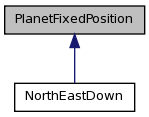
\includegraphics [width=3in]{figs/pfix_inherit.png}
\caption{Planet fixed top level}
\label{fig:4}
\end{figure}

\begin{figure}[htp]
\centering
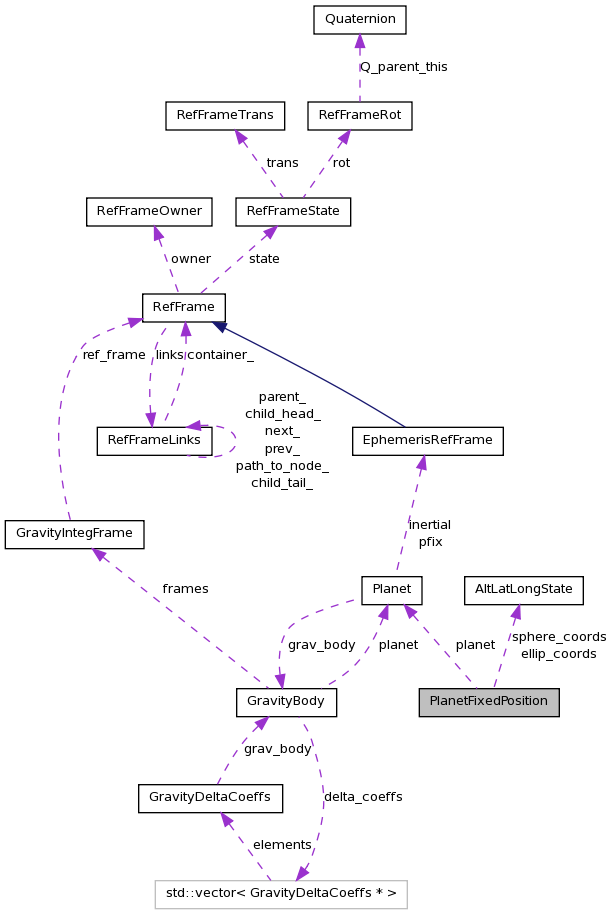
\includegraphics [width=5in]{figs/pfixcoll.png}
\caption{Planet fixed detailed }
\label{fig:5}
\end{figure}



%----------------------------------
\chapter{User Guide}\hyperdef{part}{user}{}\label{ch:user}
%----------------------------------

PLANETFIX is a utility in two modules that can be used to convert from Planet Centered Planet Fixed (PCPF) cartestian to PCPF spherical or ellipsoidal(note the nomenclature elliptical is used here for ellipsoidal)and vis versa. The second module PCPF cartesian, spherical and elliptical to a PCPF tangent plane at a given point and inversely.




\section { The analyst}
Specification of a coordinate point needs to be made:
Examples:
\begin{verbatim}

earth.cartesian_pos[0]{km} = 6778.1363e3, 0.0, 0.0;

earth.spherical_pos.altitude{M} = 1000.0;
earth.spherical_pos.latitude {d} = 45.0;
earth.spherical_pos.longitude {d} = 45.0;

earth.elliptical_pos.altitude {km} = 500.0;
earth.elliptical_pos.latitude {d} = 45.0;
earth.elliptical_pos.longitude {d} = 45.0;

or as an example conversion of PCPF to NED
set the flag
earth.ned_frame.altlatlong_type = NorthEastDown::elliptical;
input coordinates:
earth.elliptical_pos.altitude {m} = 500.0;
earth.elliptical_pos.latitude {d} = 45.0;
earth.elliptical_pos.longitude {d} = 45.0;


\end{verbatim}


\section{ SIM developers}
Builders of S\_define files and possibly input files.

\begin{verbatim}
//==============================================================================
// SIM_OBJECT: earth
// This sim object exercises the PlanetFixedPosition model.
//==============================================================================
sim_object {

   //
   // Data structures
   //

   // Structures needed for testing the full Planetary model functionality
   environment/gravity:       GravityCoeffs              gravity_coefs
      (environment/gravity/data/earth_GGM02C.d);

   environment/gravity:       GravityBody                gravity_source;

   environment/planet:        Planet                     planet
      (environment/planet/data/earth.d);

                              double                     cartesian_pos[3];
   utils/planet_fixed/planet_fixed_posn: AltLatLongState spherical_pos;
   utils/planet_fixed/planet_fixed_posn: AltLatLongState elliptical_pos;

   utils/message:             TrickMessageHandler        msg_handler;


   // Model to be tested
   utils/planet_fixed/planet_fixed_posn: PlanetFixedPosition pfix_pos;


   //
   // Initialization jobs
   //
   P_ENV (initialization) environment/gravity:
   earth.gravity_source.initialize_coefs (
      In   GravityCoeffs &      coefs        = earth.gravity_coefs);

   P_BODY (initialization) environment/planet:
   earth.planet.initialize ( );

   P_BODY (initialization) utils/planet_fixed/planet_fixed_posn:
   earth.pfix_pos.initialize (
      In   Planet *             planet_in    = &earth.planet);


   //
   // Environment class jobs
   //
   (0.0, environment) utils/planet_fixed/planet_fixed_posn:
   earth.pfix_pos.update_from_cart (
      In    const double              cart[3] = earth.cartesian_pos);

   (0.0, environment) utils/planet_fixed/planet_fixed_posn:
   earth.pfix_pos.update_from_spher (
      In    const AltLatLongState &   spher   = earth.spherical_pos);

   (0.0, environment) utils/planet_fixed/planet_fixed_posn:
   earth.pfix_pos.update_from_ellip (
      In    const AltLatLongState &   ellip   = earth.elliptical_pos);


} earth;
\end{verbatim}
For NED:
\begin{verbatim}
//==============================================================================
// SIM_OBJECT: earth
// This sim object exercises the North-East-Down model.
//==============================================================================
sim_object {

   //
   // Data structures
   //

   // Structures needed for testing the North-East-Down model functionality
   environment/gravity:       GravityCoeffs          gravity_coefs
      (environment/gravity/data/earth_GGM02C.d);

   environment/gravity:       GravityBody            gravity_source;

   environment/planet:        Planet                 planet
      (environment/planet/data/earth.d);

                              double                 cartesian_pos[3];
                              double                 cartesian_vel[3];
   utils/planet_fixed/planet_fixed_posn: AltLatLongState spherical_pos;
   utils/planet_fixed/planet_fixed_posn: AltLatLongState elliptical_pos;

   utils/message:             TrickMessageHandler    msg_handler;


   // Model to be tested
   utils/planet_fixed/north_east_down:   NorthEastDown   ned_frame;


   //
   // Initialization jobs
   //
   P_ENV (initialization) environment/gravity:
   earth.gravity_source.initialize_coefs (
      In   GravityCoeffs &      coefs        = earth.gravity_coefs);

   P_BODY (initialization) environment/planet:
   earth.planet.initialize ( );

   P_BODY (initialization) utils/planet_fixed/north_east_down:
   earth.ned_frame.initialize (
      In    Planet *            planet_in    = &earth.planet);


   //
   // Environment class jobs
   //
   (0.0, environment) utils/planet_fixed/north_east_down:
   earth.ned_frame.update_from_cart (
      In    const double              cart[3] = earth.cartesian_pos);

   (0.0, environment) utils/planet_fixed/north_east_down:
   earth.ned_frame.update_from_spher (
      In    const AltLatLongState &   spher   = earth.spherical_pos);

   (0.0, environment) utils/planet_fixed/north_east_down:
   earth.ned_frame.update_from_ellip (
      In    const AltLatLongState &   ellip   = earth.elliptical_pos);

   (0.0, environment) utils/planet_fixed/north_east_down:
   earth.ned_frame.build_ned_orientation ( );

   (0.0, environment) utils/planet_fixed/north_east_down:
   earth.ned_frame.set_ned_trans_states (
      In    double const        pos[3] = earth.cartesian_pos,
      In    double const        vel[3] = earth.cartesian_vel);


} earth;
\end{verbatim}




\section{ Model extenders} - those who are interfacing JEOD with simulations.
See the model (and it's component modules), the code and test simulations.

%----------------------------------
\chapter{Verification and Validation}\hyperdef{part}{ivv}{}\label{ch:ivv}
%----------------------------------

\section{Verification and Validation}
Introduction \newline
The following set of tests form a suite of the verification of specification
and the validation for the planet\_fixed module set(the two utility modules planet\_fixed\_posn and north\_east\_down) . The following set shows that
planet\_fixed specification are meet and thus verified.
The first set of tests is located at:
\begin{verbatim}
models/utils/planet_fixed/planet_fixed_posn/verif/SIM_PFIXPOSN_VERIF/SET_test/RUN_pfixposn_test
\end{verbatim}
They test:
\begin{enumerate}
\item Test conversion from cartesian to spherical and elliptical coordinates
\item Test conversion from spherical to cartesian and elliptical coordinates
\item Test conversion from elliptical to cartesian and spherical coordinates
\end{enumerate}

the second set is located at:
\begin{verbatim}
models/utils/planet_fixed/north_east_down/verif/SIM_NED_VERIF/SET_test/RUN_nedtest
\end{verbatim}

The validation of all these tests can be recursively verified by providing a valid fiducial set of
rectangular Cartesian or set of spheroidal geodetic coordinates. Conversely reversing the transformation to gain
the original initial conditions, the reverse transform should generate the known initial conditions.

\begin{enumerate}
\item Test conversion from cartesian to spherical and elliptical coordinates
\item Test setting of NED translational states directly
\item Test conversion from elliptical to cartesian and spherical coordinates
\end{enumerate}

The input file is a unit test configuration such that the individual module subroutines are called
from within the planet\_fixed model to execute the tests.

\subsection{Test:RUN\_pfixposn\_test }\label{pfix}
\begin{itemize}

\item{Unit Test 1}\label{unit1}:\newline
(a)Procedure:
Conversion from cartesian to spherical and elliptical coordinates
Input planet fixed coordinates:
x = 6778136.3 meters \\
y = 0.0 meters\\
z = 0.0 meters\\
Call the transformation routine at 1 second
(b) Result:
spherical altitude = 0.0 meters.\\
spherical latitude = 0.0 deg.\\
spherical longitude = 0.0 deg.\\
elliptical altitude = 0.0 deg.\\
elliptical latitude = 0.0 deg.\\
elliptical longitude = 0.0 deg.\\
(c){Pass/Fail Criterion}:\newline
The test position is located on the equator
at (equatorial radius, latitude 0 deg, long 0 deg) the
height is the same as the equatorial radius thus is zero,
the latitude and longitude , both spherical and elliptical are
by default zero. The test is passed.

\item{Unit Test 2}:\label{unit2} \newline
(a)Procedure:
Test conversion from spherical to cartesian and elliptical coordinates
Input planet fixed coordinates at 2 seconds :
spherical altitude = 1000.0 meters\\
spherical latitude = 3.1416 radians (or 180 degrees)\\
spherical longitude = 1.0 (radian), (or 57.2957795 degrees)\\
Call the transformation routine at 1 second.\\
(b) Result:\\
x  = 6.778136e+06 meters.\\
y  = 0.0 meters\\
z  = 0.0 meters\\
elliptical altitude = 1.159497e-06 meters.\\
elliptical latitude = -4.237551e-04 deg.\\
elliptical longitude = -1.227042e+02  deg.\\
(c){Pass/Fail Criterion}:\newline
The initial values given in this test were computed independently
using FORTRAN routines supplied by Vallado \cite{VMcc} and Borkowski \cite{bor}
and found to differ by only about .5 meters and .3 degrees, since these are more
sophisticated methods the results are considered in good agreement.
The test is passed.

\item{Unit Test 3}:\label{unit3}\newline
Test conversion from elliptical to cartesian and spherical coordinates
(a)Procedure:\newline
Test conversion from elliptical to cartesian and spherical coordinates
Input planet fixed coordinates:
elliptical altitude = 500.0 meters.\\
elliptical latitude = 5.729578e+01 deg.\\
elliptical longitude = 1.800004e+02  deg\\
Call the transformation routine at 1 second\\
(b) Result:\newline
x  = -3454588.934 meters.\\
y  = -25.378827 meters\\
z  = 5344189.181 meters\\
spherical altitude = -1.460475e+04 meters.\\
spherical latitude = 5.712058e+01  deg.\\
spherical longitude = -1.799996e+02 deg.\\
(c){Pass/Fail Criterion}:\newline
The initial values given in this test were computed independently
using FORTRAN routines supplied by Vallado \cite{VMcc} and Borkowski \cite{bor}
and found to differ by only about .5 meters and .3 degrees. These more
sophisticated methods the produce results that are considered in good agreement
with the JEOD unit test above.
The test is passed.


\end{itemize}

\subsection{Test:RUN\_nedtest }\label{ned}
\begin{itemize}
\item{Unit Test 1}:\label{unit4}\newline
a)Procedure:\newline
Test setting of NED translational states directly :\newline
Input:\\
x= 6778136.3 meters \\
y= 0.0 meters\\
z= 0.0 meters \\
(b)Result both spherical and elliptical:\\
Geodetic height = 399999.3 meters \\
Latitude = 0.0 degrees \\
Longitude = 0.0 degrees \\
(c){Pass/Fail Criterion}:\newline
The height is the difference between the radius given and the Earth's mean equatorial radius.
The location is the prime meridian thus the longitude and latitude are (0,0)
The test passes the success criterion.

\item{Unit Test 2}:\label{unit5}\newline
a)Procedure:\newline
Test conversion from cartesian to spherical and elliptical coordinates, as
well as setting of translational (pos/vel) states based on conversion:\newline
Input\\
x= 6778136.3 meters \\
y= 0.0 meters\\
z= 0.0 meters \\
vx = 0.0 m/s \\
vy = 100 m/s \\
vz = 700 m/s \\
(b)Result both spherical and elliptical\\
Geodetic height = 399999.3 meters \\
Latitude = 0.0 degrees \\
Longitude = 0.0 degrees \\
vxned = 0.0 m/s \\
vyned = 100.0 m/s \\
vzned = -700.0 m/s \\
(c){Pass/Fail Criterion}:\newline
The geodetic height is same as unit test 1.\\
The transform matrix is:
\begin{equation}
\left[ {\begin{array}{*{20}c}
   0 & 0 & 1  \\
   0 & 1 & 0  \\
   0 & 0 & { - 1}  \\
\end{array}} \right]
\end{equation}
by hand calculation the resulting tangential coordinates are correct
and the test is passed.

\item{Unit Test 3}: \label{unit6} \newline
a)Procedure:\newline
Test conversion from spherical to cartesian and elliptical coordinates, as
well as setting of frame's orientation states based on conversion
Input spherical\\
altitude = 1000.0 m;\\
latitude = 3.1416 r;\\
longitude = 1.0 r;\\
(b)Result (NED-Cartesians)\\
x= -3446122 meters \\
y= -5367017  meters\\
z= -46.86 meters \\
(c){Pass/Fail Criterion}:\newline
Since one does not need to iterate for latitude the results can calculated by hand
using equations (3.20), the results are same and the test validated.

\item{Unit Test 4}: \label{unit7} \newline
a)Procedure:\newline
Test conversion from elliptical to cartesian and spherical coordinates, as
well as setting of frame's orientation states based on conversion
Input elliptical
altitude = 500.0 m \\
latitude = 1.0 r \\
longitude = 3.1416 r\\
(b)Result\\
xned = -3454588.934 m \\
yned = -25.3788 m \\
zned = 5344189.181 m \\

(c){Pass/Fail Criterion}:
\end{itemize}
This test is hard to verify by hand.
An independent check with an example in the book Global Positioning System and Inertial Navigation \cite{far}
was input into the JEOD utility routine. From an example in chapter 2 the following is input and the planet\_fixed
module for this conversion was check by an independent simulation:
\begin{equation}
\left[ {\begin{array}{*{20}c}
   {\lambda (longitude}  \\
   {\phi (latitude)}  \\
   {h(height)}  \\
\end{array}} \right] = \left[ {\begin{array}{*{20}c}
   {.59341195(radians)}  \\
   { - 2.0478571(radians)}  \\
   {251.702(meteres)}  \\
\end{array}} \right]
\end{equation}
With the resulting transformation:
\begin{equation}
\left[ {\begin{array}{*{20}c}
   {x_{ned} }  \\
   {y_{ned} }  \\
   {z_{ned} }  \\
\end{array}} \right] = \left[ {\begin{array}{*{20}c}
   { - 2,430,601.8}  \\
   { - 4,702,442.7}  \\
   {3,546,587.4}  \\
\end{array}} \right]\left( {meters} \right)
\end{equation}
Therefore the algorithm is verified.



\chapter{Requirements Traceability}\label{sec:traceability}
\begin{table}[htp]
\centering
\caption{planet\_fixed Traceability - Tests}
\vspace{1ex}
\begin{tabular}{|l|l|}
\hline
\multicolumn{2}{|c|}{Requirments and Tests} \\
\hline
 Planet fixed Cartesian \ref{reqt:pfixcart}  ~& Test \ref{unit1} and Test \ref{unit2} \\
 Planet fixed spherical \ref{reqt:sphere} ~& Test \ref{unit2}  and Test \ref{unit1}\\
 Planet fixed Elliptical \ref{reqt:pfixellip}  ~& Test \ref{unit3}  and Test \ref{unit4}\\
 Planet fixed tangent plane \ref{reqt:pfixtan}  ~& Test \ref{unit5} and Test  \ref{unit6} and Test \ref{unit7} \\
\hline
\end{tabular}
\end{table}


\newpage
%%%%%%%%%%%%%%%%%%%%%%%%%%%%%%%%%%%%%%%%%%%%%%%%%%%%%%%%%%%%%%%%%%%%%%%%%
% Appendix
%%%%%%%%%%%%%%%%%%%%%%%%%%%%%%%%%%%%%%%%%%%%%%%%%%%%%%%%%%%%%%%%%%%%%%%%%
\appendix
\appendixpage
\addappheadtotoc
\chapter{S\_define Unit Test One}\label{ap1:s1}
\begin{verbatim}
//==============================================================================
// This simulation is a demonstration Trick simulation for exercising the base
// planet-fixed position model in JEOD. The following simulation objects are
// defined in this sim:
//
//          sys - Trick runtime executive and data recording routines
//         time - Universal time
//        earth - Object used to exercise planet-fixed position model
//
//==============================================================================


// Define job calling intervals
#define ENVIRONMENT     1.00   // Ephemeris update interval


// Define the phase initialization priorities.
// NOTE: Initialization jobs lacking an assigned phase initialization priority
// run after all initialization jobs that have assigned phase init priorities.
#define P_TIME  P10   // Highest priority; these jobs only depend on time
#define P_ENV   P20   // Environment initializations
#define P_BODY  P30   // Orbital body initializations



//==============================================================================
// SIM_OBJECT: sys
// This is the Trick executive model; this model should be basically
// the same for all Trick applications.
//==============================================================================
sim_object {

   //
   // Data structures
   //

   sim_services/include: EXECUTIVE exec (sim_services/include/executive.d);


   //
   // Automatic jobs
   //

   sim_services/input_processor: input_processor (
      Inout INPUT_PROCESSOR *IP = &sys.exec.ip);

} sys;



//==============================================================================
// SIM_OBJECT: time
// This sim object relates simulation time to time on the Earth.
//==============================================================================
sim_object {

   //
   // Data structures
   //
   environment/time: TimeManager time_manager;
   environment/time: TimeManagerInit time_manager_init;

   //
   // Initialization jobs
   //
   P_TIME (initialization)  environment/time: time.time_manager.initialize(
      Inout TimeManagerInit * time_manager_init = &time.time_manager_init);

   //
   // Scheduled jobs
   //
   (ENVIRONMENT, environment) environment/time: time.time_manager.update(
      In    double            simtime           = sys.exec.out.time);

} time;



//==============================================================================
// SIM_OBJECT: earth
// This sim object exercises the PlanetFixedPosition model.
//==============================================================================
sim_object {

   //
   // Data structures
   //

   // Structures needed for testing the full Planetary model functionality
   environment/gravity:       GravityCoeffs              gravity_coefs
      (environment/gravity/data/earth_GGM02C.d);

   environment/gravity:       GravityBody                gravity_source;

   environment/planet:        Planet                     planet
      (environment/planet/data/earth.d);

                              double                     cartesian_pos[3];
   utils/planet_fixed/planet_fixed_posn: AltLatLongState spherical_pos;
   utils/planet_fixed/planet_fixed_posn: AltLatLongState elliptical_pos;

   utils/message:             TrickMessageHandler        msg_handler;


   // Model to be tested
   utils/planet_fixed/planet_fixed_posn: PlanetFixedPosition pfix_pos;


   //
   // Initialization jobs
   //
   P_ENV (initialization) environment/gravity:
   earth.gravity_source.initialize_coefs (
      In   GravityCoeffs &      coefs        = earth.gravity_coefs);

   P_BODY (initialization) environment/planet:
   earth.planet.initialize ( );

   P_BODY (initialization) utils/planet_fixed/planet_fixed_posn:
   earth.pfix_pos.initialize (
      In   Planet *             planet_in    = &earth.planet);


   //
   // Environment class jobs
   //
   (0.0, environment) utils/planet_fixed/planet_fixed_posn:
   earth.pfix_pos.update_from_cart (
      In    const double              cart[3] = earth.cartesian_pos);

   (0.0, environment) utils/planet_fixed/planet_fixed_posn:
   earth.pfix_pos.update_from_spher (
      In    const AltLatLongState &   spher   = earth.spherical_pos);

   (0.0, environment) utils/planet_fixed/planet_fixed_posn:
   earth.pfix_pos.update_from_ellip (
      In    const AltLatLongState &   ellip   = earth.elliptical_pos);


} earth;

\end{verbatim}

\chapter{Input file for Unit Test 1}\label{ap2:in1}

\begin{verbatim}

/*******************************************************************************
   Purpose:   Input file used for JEOD NorthEastDown model unit test

   Test:      Verify all methods of NorthEastDown work correctly

*******************************************************************************/

#define LOG_CYCLE 0.10

// Default data file generated in S_define
#include "S_default.dat"

// Set up simulation executive parameters
sys.exec.in.trap_sigfpe = Yes;

// Set up parameters to record
#include "Log_data/log_ned_verif.d"


// Set pointers between test planet and test grav_source
earth.planet.grav_source = &earth.gravity_source;
earth.gravity_source.planet = &earth.planet;


/* Test conversion from cartesian to spherical and elliptical coordinates, as
   well as setting of translational (pos/vel) states based on conversion */
read = 1.0;
earth.cartesian_pos[0] = 6778.1363e3, 0.0, 0.0;
call earth.earth.ned_frame.update_from_cart (earth.cartesian_pos);


// Test setting of NED translational states directly
read = 2.0;
earth.cartesian_pos[0] = 6778.1363e3, 0.0, 0.0;
earth.cartesian_vel[0] = 0.0, 100.0, -750.0;
call earth.earth.ned_frame.set_ned_trans_states (earth.cartesian_pos);


/* Test conversion from spherical to cartesian and elliptical coordinates, as
   well as setting of frame's orientation states based on conversion */
read = 3.0;
earth.spherical_pos.altitude = 1000.0;
earth.spherical_pos.latitude = 3.1416;
earth.spherical_pos.longitude = 1.0;
call earth.earth.ned_frame.update_from_spher (earth.spherical_pos);
earth.ned_frame.altlatlong_type = NorthEastDown::spherical;
call earth.earth.ned_frame.build_ned_orientation ();


// Reset enum defining the spherical/elliptical basis for N-E-D definition
read = 3.5;
earth.ned_frame.altlatlong_type = NorthEastDown::undefined;


/* Test conversion from elliptical to cartesian and spherical coordinates, as
   well as setting of frame's orientation states based on conversion */
read = 4.0;
earth.elliptical_pos.altitude = 500.0;
earth.elliptical_pos.latitude = 1.0;
earth.elliptical_pos.longitude = 3.1416;
call earth.earth.ned_frame.update_from_ellip (earth.elliptical_pos);
earth.ned_frame.altlatlong_type = NorthEastDown::elliptical;
call earth.earth.ned_frame.build_ned_orientation ();


// End simulation
stop = 5.0;
\end{verbatim}

\chapter{S\_define Unit Test Two}\label{ap3:s2}
\begin{verbatim}
//==============================================================================
// This simulation is a demonstration Trick simulation for exercising the JEOD
// North-East-Down model. The following simulation objects are defined in
// this sim:
//
//          sys - Trick runtime executive and data recording routines
//         time - Universal time
//        earth - Object used to exercise the North-East-Down model
//
//==============================================================================


// Define job calling intervals
#define ENVIRONMENT     1.00   // Environment update interval


// Define the phase initialization priorities
/* NOTE: Initialization jobs lacking an assigned initialization priority run
   after all initialization jobs that have assigned phase init priorities. */
#define P_TIME  P10   // Highest priority; these jobs only depend on time
#define P_ENV   P20   // Environment initializations
#define P_BODY  P30   // Orbital body initializations



//==============================================================================
// SIM_OBJECT: sys
// This is the Trick executive model; this model should be basically
// the same for all Trick applications.
//==============================================================================
sim_object {

   //
   // Data structures
   //
   sim_services/include: EXECUTIVE exec (sim_services/include/executive.d);

   //
   // Automatic jobs
   //
   sim_services/input_processor: input_processor (
      Inout INPUT_PROCESSOR *IP = &sys.exec.ip);

} sys;



//==============================================================================
// SIM_OBJECT: time
// This sim object relates simulation time to time on the Earth.
//==============================================================================
sim_object {

   //
   // Data structures
   //
   environment/time: TimeManager time_manager;
   environment/time: TimeManagerInit time_manager_init;

   //
   // Initialization jobs
   //
   P_TIME (initialization)  environment/time: time.time_manager.initialize(
      Inout TimeManagerInit * time_manager_init = &time.time_manager_init);

   //
   // Scheduled jobs
   //
   (ENVIRONMENT, environment) environment/time: time.time_manager.update(
      In    double            simtime           = sys.exec.out.time);

} time;



//==============================================================================
// SIM_OBJECT: earth
// This sim object exercises the North-East-Down model.
//==============================================================================
sim_object {

   //
   // Data structures
   //

   // Structures needed for testing the North-East-Down model functionality
   environment/gravity:       GravityCoeffs          gravity_coefs
      (environment/gravity/data/earth_GGM02C.d);

   environment/gravity:       GravityBody            gravity_source;

   environment/planet:        Planet                 planet
      (environment/planet/data/earth.d);

                              double                 cartesian_pos[3];
                              double                 cartesian_vel[3];
   utils/planet_fixed/planet_fixed_posn: AltLatLongState spherical_pos;
   utils/planet_fixed/planet_fixed_posn: AltLatLongState elliptical_pos;

   utils/message:             TrickMessageHandler    msg_handler;


   // Model to be tested
   utils/planet_fixed/north_east_down:   NorthEastDown   ned_frame;


   //
   // Initialization jobs
   //
   P_ENV (initialization) environment/gravity:
   earth.gravity_source.initialize_coefs (
      In   GravityCoeffs &      coefs        = earth.gravity_coefs);

   P_BODY (initialization) environment/planet:
   earth.planet.initialize ( );

   P_BODY (initialization) utils/planet_fixed/north_east_down:
   earth.ned_frame.initialize (
      In    Planet *            planet_in    = &earth.planet);


   //
   // Environment class jobs
   //
   (0.0, environment) utils/planet_fixed/north_east_down:
   earth.ned_frame.update_from_cart (
      In    const double              cart[3] = earth.cartesian_pos);

   (0.0, environment) utils/planet_fixed/north_east_down:
   earth.ned_frame.update_from_spher (
      In    const AltLatLongState &   spher   = earth.spherical_pos);

   (0.0, environment) utils/planet_fixed/north_east_down:
   earth.ned_frame.update_from_ellip (
      In    const AltLatLongState &   ellip   = earth.elliptical_pos);

   (0.0, environment) utils/planet_fixed/north_east_down:
   earth.ned_frame.build_ned_orientation ( );

   (0.0, environment) utils/planet_fixed/north_east_down:
   earth.ned_frame.set_ned_trans_states (
      In    double const        pos[3] = earth.cartesian_pos,
      In    double const        vel[3] = earth.cartesian_vel);


} earth;

\end{verbatim}

\chapter{Input file for Unit Test 2}\label{ap4:in2}

\begin{verbatim}
/*******************************************************************************
   Purpose:   Input file used for JEOD NorthEastDown model unit test

   Test:      Verify all methods of NorthEastDown work correctly

*******************************************************************************/

#define LOG_CYCLE 0.10

// Default data file generated in S_define
#include "S_default.dat"

// Set up simulation executive parameters
sys.exec.in.trap_sigfpe = Yes;

// Set up parameters to record
#include "Log_data/log_ned_verif.d"


// Set pointers between test planet and test grav_source
earth.planet.grav_source = &earth.gravity_source;
earth.gravity_source.planet = &earth.planet;


/* Test conversion from cartesian to spherical and elliptical coordinates, as
   well as setting of translational (pos/vel) states based on conversion */
read = 1.0;
earth.cartesian_pos[0] = 6778.1363e3, 0.0, 0.0;
call earth.earth.ned_frame.update_from_cart (earth.cartesian_pos);


// Test setting of NED translational states directly
read = 2.0;
earth.cartesian_pos[0] = 6778.1363e3, 0.0, 0.0;
earth.cartesian_vel[0] = 0.0, 100.0, -750.0;
call earth.earth.ned_frame.set_ned_trans_states (earth.cartesian_pos);


/* Test conversion from spherical to cartesian and elliptical coordinates, as
   well as setting of frame's orientation states based on conversion */
read = 3.0;
earth.spherical_pos.altitude = 1000.0;
earth.spherical_pos.latitude = 3.1416;
earth.spherical_pos.longitude = 1.0;
call earth.earth.ned_frame.update_from_spher (earth.spherical_pos);
earth.ned_frame.altlatlong_type = NorthEastDown::spherical;
call earth.earth.ned_frame.build_ned_orientation ();


// Reset enum defining the spherical/elliptical basis for N-E-D definition
read = 3.5;
earth.ned_frame.altlatlong_type = NorthEastDown::undefined;


/* Test conversion from elliptical to cartesian and spherical coordinates, as
   well as setting of frame's orientation states based on conversion */
read = 4.0;
earth.elliptical_pos.altitude = 500.0;
earth.elliptical_pos.latitude = 1.0;
earth.elliptical_pos.longitude = 3.1416;
call earth.earth.ned_frame.update_from_ellip (earth.elliptical_pos);
earth.ned_frame.altlatlong_type = NorthEastDown::elliptical;
call earth.earth.ned_frame.build_ned_orientation ();


// End simulation
stop = 5.0;

\end{verbatim}


%%%%%%%%%%%%%%%%%%%%%%%%%%%%%%%%%%%%%%%%%%%%%%%%%%%%%%%%%%%%%%%%%%%%%%%%%
% Bibliography
%%%%%%%%%%%%%%%%%%%%%%%%%%%%%%%%%%%%%%%%%%%%%%%%%%%%%%%%%%%%%%%%%%%%%%%%%

\newpage
\pdfbookmark{Bibliography}{bibliography}
\bibliography{dynenv,PLANETFIX}
\bibliographystyle{plain}

\end{document}
